\documentclass{article}
\usepackage[utf8]{inputenc}
\usepackage{graphicx}
\usepackage{amsmath}
\usepackage{amssymb}
\usepackage{tikz}

\setlength{\parindent}{0pt}
\usepackage[letterpaper, margin=1.0in]{geometry}

\title{MATH 116: Final Exam Review}
\author{Sam Boardman}
\date{December 4, 2024}

\begin{document}

\maketitle

The following problems may be attempted in any order based on which concepts you would most like to review. Problems marked by (\textasteriskcentered{}) are more challenging (or more abstract) than questions likely to appear on an exam for MATH 116.   

\begin{enumerate}

\item Sam's elementary school, being located on New Jersey's coastline, made prominent use of a wave design, plastering it on t-shirts, yearbooks, and cups (that turned purple upon introduction to liquid). The design can be described as the region in the first quadrant bounded by the polar curves $$r = 1 + \sin(\theta)\cos(2\theta)$$ and $$r = 2\cos(\theta),$$ where all distances are measured in decimeters. Each of these curves is plotted below in the first quadrant:

\begin{center}
  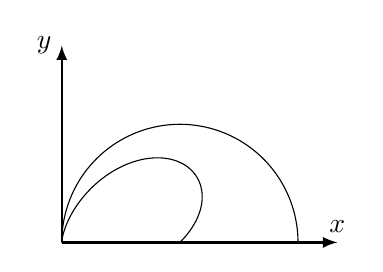
\begin{tikzpicture}[xscale=1,yscale=1]
  \draw[thick,->,>=latex] (0,0)--(3.5,0) node[above] {$x$};
  \draw[thick,->,>=latex] (0,0)--(0,2.5) node[left] {$y$};
  \draw[domain=0:90,scale=1.5,samples=500] plot (\x:{2*cos(\x)});
  \draw[domain=0:90,scale=1.5,samples=500] plot (\x:{1+sin(\x)*cos(\x/.5)});
  \end{tikzpicture}
  \end{center}

\begin{enumerate}
    \item Find the area of the design. Include units.

    \vfill
    
    \item Find the perimeter of the design. Include units. 

    \vfill 
\end{enumerate}

\newpage

\item (\textasteriskcentered{}) While not always excited to wake up and ``rid[e] the waves of excellence" on weekdays, Sam readily got up at 7am on Saturdays for a day of unmitigated indulgence, starting with a trip to the town's premier (and only) deli. There, Sam liked to operate the coffee machine for his mom, but oscillated between two extremes (based on a good-faith interpretation of the feedback he received): very small additions to the cup and very large additions to the cup. \\

Let $s_n = \begin{cases} \frac{9\sin(\frac{1}{n})}{n} & \text{if } n \text{ is odd} \\ \frac{\sin(\frac{1}{n})}{n} & \text{if } n \text{ is even} \end{cases}$ be the amount of coffee (in ounces) in the $n$th squirt added to the cup. Is the total amount of coffee added to the cup finite? Justify your answer.       

\vfill

% His mom would drive him there, but they did not take the same amount of time to get ready in the morning, resulting in each completing miscellaneous tasks while waiting for the other. Let $s_n$ and $v_n$ denote the time required (in minutes) for the $n$th task completed by Sam and Vicki, respectively; $n = 1$ corresponds to getting ready in the morning, which commences at 7am. 

% \begin{enumerate}
%    \item Suppose $\sum_{n=1}^\infty s_n$ and $\sum_{n=1}^\infty v_n$ converge. Is is true that there is a time after 7am such that neither are in the middle of a task?
%    \item Suppose $s_n = 7\cdot(1/2)^{n-1}$ and $v_n = 10\cdot(1/20)^{n-1}$. Find the first time after 7am such that neither are in the middle of a task.
% \end{enumerate}

\item (\textasteriskcentered{}) After completing Calculus 2 (yes, it was challenging), Sam traded ocean for forest and went to Cornell, where he learned many cool facts about integrals. One of them is that a function $f(x)$ with domain $a \leq x \leq b$ is \textit{integrable} (i.e. all Riemann sums of $f(x)$ on $[a,b]$ converge to the same value, which we call the definite integral $\int_a^b f(x)dx$) if and only if $f(x)$ is bounded and the set of points at which $f(x)$ is discontinuous has measure zero. We say a set has \textit{measure zero} if it can be covered by intervals $(a_1,b_1),(a_2,b_2),\dots$ such that the sum of their lengths $\sum_{n=1}^\infty (b_n-a_n)$ is as close to 0 as we want. \\ 

For example, $g(x) = \begin{cases} \sin x, & 0 \leq x \leq .5 \\ x^2, & .5 < x \leq 1 \end{cases}$ is integrable since it is only discontinuous at $x = .5$, which can be covered by the interval $(.45,.55)$ of length .1, or the interval $(.495,.505)$ of length .01, and so on. On the other hand, $h(x) = \begin{cases} 0, & x = 0 \\ \frac{1}{\sqrt{x}}, & 0 < x \leq 1 \end{cases}$ is not integrable since it has a vertical asymptote (hence the need for the notion of improper integrals). \\

Let $f(x)$ be a bounded function with domain $a \leq x \leq b$ that is piecewise continuous; it is only discontinuous at the points $x = c_1,c_2,\dots$. Show that $f(x)$ is integrable.

\vfill 

\newpage

\item All this learning about integrals required a lot of studying while on the hill. Seeking periods of sustained concentration between collaborations, Sam sometimes preferred to work in relative quiet, including whilst walking. Fortunately, the campus becomes more sparsely populated as one walks East on Tower Road. Let $x$ be the distance (in meters) from the Western terminus of Tower Road (which, paradoxically, is East Ave) and $\delta(x)$ the corresponding people density (in people per meter) at that point.

\begin{enumerate}
    \item Suppose Sam starts at East Ave and would like to find a spot along Tower Road to study. Given a point $x$ as above, find an expression for the sum $S(x)$ of its people density (in people per meter) and the number of people Sam has to walk past to get there. Your answer may involve $\delta(x)$ and one or more integrals. 

    \vfill

    \item Let $\delta(x) = 100e^{-2x}$. Is $S(x)$ decreasing for $x > 0$? Justify your answer using calculus.   

    \vfill 
\end{enumerate}

\item Worried that quiet contemplation of esoteric math facts will eventually ring hollow beyond the realm of adversarially dispensed coffee and excursions to clock towers, Sam begins preparing for internship interviews. One of the questions he encounters asks for the average number of cards that must be drawn from a 52-card deck to get an ace (of which there are 4 in the deck). For $n \geq 4$, let $A_n$ be the average number of cards that must be drawn from a $n$-card deck to get an ace (letting the deck still have 4 aces). After some experimentation, Sam discovers the following recursive formula:

$$A_{n+1} = A_n + \frac{1}{5}, n \geq 4.$$

Calculate the average number of cards that must be drawn from a 52-card deck to get an ace. 

\vfill

\end{enumerate}

\end{document}
